\chapter{Current defense mechanisms}
\label{chp:current-defense-mechanisms}

This chapter provides information about defense mechanisms trying to mitigate stack buffer overflow attacks as they are currently employed by the Linux kernel or the compiler.
This refers to software versions as described in \cref{sec:system-model}.

\Cref{chp:attack-vectors} then describes the actual attack possibilities that arise from a stack buffer overflow vulnerability and how such attack vectors can be rendered unusable or at least inefficient and hard to exploit.

Additionally, some of the attacks described in \cref{chp:attack-vectors} can also be used to bypass some of the mitigation measures described in \hyperref[chp:current-defense-mechanisms]{this \namecref{chp:current-defense-mechanisms}}.
Therefore, \cref{chp:defense-mechanism-improvements} provides different approaches on how to improve the defense mechanisms in order to prevent even more attacks.

\section{Compiler-based measures}
\label{sec:compiler-based-measures}

Depending on compiler options and flags, the compiled binary output can differ greatly.
Some measures which help mitigate stack buffer overflows are presented in the following sections.

\subsection{The \texttt{\_FORTIFY\_SOURCE} macro}
\label{subsec:fortify-source}

Support for the \texttt{\_FORTIFY\_SOURCE} macro was added to \gls{gcc} in \citedate{Jelinek2004} and is available since \gls{gcc} version 4.0 \cite{Sharma2014}.
The possible values for this macro are 0, 1 and 2 with 0 meaning that it has no effect and 2 meaning that all measures that are implied by this macro are active.

The effect of this macro is that the compiler checks at compile time as well as at runtime whether a destination buffer is overflown by functions such as \texttt{strcpy}, \texttt{strncat}, \texttt{memcpy}, and so forth%
	\footnote{Supported functions according to \cite{Kerrisk2020,Sharma2014}: \texttt{memcpy, mempcpy, memmove, memset, strcpy, stpcpy, strncpy, strcat, strncat, sprintf, vsprintf, snprintf, vsnprintf, gets}}%
.
In order to achieve this, the compiler checks at compile time whether the destination is big enough to hold the source's contents.
This is done by comparing function arguments (e.g. the number of bytes to set in \texttt{memset}) or array sizes, if the source and destination arrays have fixed sizes.
If the compiler detects an overflow, it issues a warning \cite{Jelinek2004,Kerrisk2020,Sharma2014,Sidhpurwala2018}.

For dynamic sized operands where the compiler cannot determine whether the destination operand will be overflown, the function calls are replaced with wrapper functions that check the operands' sizes.
For example, \texttt{strcpy} is replaced with \texttt{\_\_strcpy\_chk}.
If the check fails, the program execution is aborted with an error message \cite{Kerrisk2020,Sharma2014}.

The \texttt{\_FORTITY\_SOURCE} macro can either be manually set to a value higher than 0 or is automatically activated when compiler optimizations are enabled, for example by passing the \texttt{-O3} flag to \gls{gcc} \cite{Kerrisk2020,Sharma2014,Sidhpurwala2018}.
\todo{Include example? Not sure}

\citeauthor{Jelinek2004} states in the announcement of the original implementation of this feature that the runtime overhead of the checks is very small and that the compiler automatically omits the checks if it can prove at compile time that no overflow can occur \cite{Jelinek2004}.

\subsection{Optimizing compilation}
\label{subsec:optimizing-compilation}

With compiler optimizations enabled (for example by passing the \texttt{-O3} flag), \gls{gcc} compiles code differently which might make a buffer overflow unusable.
In the example seen in \cref{lst:optimization,lst:optimization-disassembly,lst:optimization-disassembly-optimized}, a stack buffer overflow vulnerability lies in the function \texttt{copy}, as a string is copied into an 8 byte stack buffer without checking for the size.

\lstinputlisting[language=C,float=ht,caption={C program copying \texttt{argv[1]} into a function-local buffer},label={lst:optimization}]{code/optimization.c}

\begin{lstlisting}[language=bash,float=ht,caption={Disassembly excerpt of the 64 bit binary compiled from the code in \cref{lst:optimization} with \texttt{gcc -o copy optimization.c -fno-stack-protector}, retrieved with \texttt{objdump -D -{}-no-show-raw-insn copy}}, label={lst:optimization-disassembly}]
0000000000001149 <copy>:
1149:       push   %rbp
114a:       mov    %rsp,%rbp
114d:       sub    $0x20,%rsp
1151:       mov    %rdi,-0x18(%rbp)
1155:       mov    -0x18(%rbp),%rdx
1159:       lea    -0x8(%rbp),%rax
115d:       mov    %rdx,%rsi
1160:       mov    %rax,%rdi
1163:       callq  1030 <strcpy@plt>
1168:       nop
1169:       leaveq
116a:       retq

000000000000116b <main>:
116b:       push   %rbp
116c:       mov    %rsp,%rbp
116f:       sub    $0x10,%rsp
1173:       mov    %edi,-0x4(%rbp)
1176:       mov    %rsi,-0x10(%rbp)
117a:       mov    -0x10(%rbp),%rax
117e:       add    $0x8,%rax
1182:       mov    (%rax),%rax
1185:       mov    %rax,%rdi
1188:       callq  1149 <copy>
118d:       mov    $0x0,%edi
1192:       callq  1040 <exit@plt>
1197:       nopw   0x0(%rax,%rax,1)
\end{lstlisting}

\begin{lstlisting}[language=bash,float=ht,caption={Disassembly excerpt of the 64 bit binary compiled from the code in \cref{lst:optimization} with \texttt{gcc -o copy optimization.c -fno-stack-protector -O3}, retrieved with \texttt{objdump -D -{}-no-show-raw-insn copy}}, label={lst:optimization-disassembly-optimized}]
0000000000001050 <main>:
1050:       sub    $0x18,%rsp
1054:       mov    0x8(%rsi),%rsi
1058:       lea    0x8(%rsp),%rdi
105d:       callq  1030 <strcpy@plt>
1062:       xor    %edi,%edi
1064:       callq  1040 <exit@plt>
1069:       nopl   0x0(%rax)
\end{lstlisting}

\Cref{lst:optimization-disassembly} shows the compiler output without optimizations enabled.
It inhibits the expected behavior: \texttt{main} calls \texttt{copy}, \texttt{copy} increases the stack size to hold the 8 byte buffer and then copies the string handed to the function into said buffer.
This allows to overflow the buffer and thus overwrite \gls{sfp} and \gls{rip} with user-controlled data.
When \texttt{copy} then returns, the program continues execution at the user-controlled location.

\Cref{lst:optimization-disassembly-optimized} in contrast shows the compiler output with optimizations enabled.
The compiler performs several optimizations.
For example, it omits the usage of the \texttt{rbp} register and does not address relative to the stack frame base but to the stack pointer.
The main point, however, here is that the \texttt{copy} function is inlined, meaning that the necessary instructions are directly included in \texttt{main} instead of \texttt{main} calling \texttt{copy}.
This still allows to overflow the buffer, which is now located on \texttt{main}'s stack frame.
However, as \texttt{main} never returns but directly calls \texttt{exit}, there is no \gls{rip} to overwrite in order to gain control over the execution flow.

Thus, in the given example, enabling compiler optimizations can prevent an attacker from diverting control flow.

In general, this is not always the case.
Not all functions are inlined and not in any case an attacker just wants to overwrite the \gls{rip} or \texttt{main} never returns.
Thus, compiler optimizations should not be seen as a measure to prevent attackers from exploiting stack buffer overflows.
They can make such vulnerabilities harder to exploit in certain cases but not mitigate them in total.

There are a lot of further compiler optimizations which influence the stack layout or the code generation.
However, listing and explaining all of them would exceed the scope of this paper and is thus not included here.

\section{Executable space protection}
\label{sec:executable-space-protection}

As mentioned in \cref{sec:stack-buffer-overflows}, the mixture of control flow information and data on the stack is what enables attackers to exploit stack buffer overflow vulnerabilities in order to divert control flow.
Because the stack contents are often user-controlled, for example when saving command line input on the stack, a measure of protection against executing previously written code is a possibility to harden a system against stack buffer overflows.
Such protections are often referred to as \emph{executable space protection} or \emph{\gls{dep}}, where the latter term is often used for Microsoft Windows specific implementations \cite{Satran2018}.

On 64 bit machines, memory pages are marked with specific flags signaling the permissions for the given memory page.
Those flags include a \gls{nx} bit (marketed as \gls{xd} bit by Intel) \cite[801\psq]{Bryant2011}.
If set to 1, this bit informs the processor that the marked memory page should not contain executable code and that accesses to such pages trying to execute code should throw an exception (\acl{segfault}).
On 32 bit machines, such a bit was only emulated in software instead of implemented in hardware, as it is part of the \gls{pae} enabling 32 bit machines to use more than 4 GiB of memory \cite{Molnar2004}.
The Linux kernel makes use of the \gls{nx} bit by default since \citeyear{Cook2010} \cite{Cook2010}.

These flags allows marking specific pages as non-executable, such as the memory pages containing a program's stack.
Furthermore, a \gls{wxorx} approach on modern systems marks memory pages as either writable or executable but not both at the same time.
This approach can be seen as an extension to just marking the stack as non-executable and prevents an attacker from executing code he has written into the program's memory space before.

\section{Function pointer protection}
\label{sec:function-pointer-protection-current}

Buffer overflows can not only affect the \acrfull{sfp} and \acrfull{rip} but also other stack contents such as function pointers.
Thus, an attacker can also divert control flow if they manage to overwrite a function pointer instead of the \gls{rip} and the program tries to call the corresponding function through such a function pointer afterwards.

In order to make such attacks harder to achieve, \gls{glibc} implements a function pointer mangling macro, \texttt{PTR\_MANGLE} and the corresponding counterpart, \texttt{PTR\_DEMANGLE}.
Those macros hide function pointer values by applying a XOR operation with a per-process randomized value%
	\footnote{For an example on how this preprocessor macro can be used, see the \texttt{setjmp} sources on \href{https://sourceware.org/git/?p=glibc.git;a=blob;f=sysdeps/x86_64/setjmp.S;h=b4e05e0f0c1bb2184cf872a6a26eb18de6cfeba1;hb=9ea3686266dca3f004ba874745a4087a89682617}{sourceware.org}.}
\cite{Newton2013}.
An attacker cannot just overwrite the mangled function pointer because the overwritten value would be turned into an unusable junk on demangling the pointer with the unknown value.
Thus, an attacker would have to somehow get hold of the secret value used for mangling and demangling pointers before creating their own mangled pointer.

It is, however, important to note that such pointer mangling is not automatically conducted for any function pointers but that it is a \gls{glibc} internal macro used in \gls{glibc} in some cases.

\section{\glsentrylong{aslr} (\glsentryshort{aslr})}
\label{sec:aslr-and-pie}

\gls{aslr} and \acrfull{pie} are some measures which were introduced to make it harder for an attacker to hit the correct address when overwriting function pointers or the \gls{rip}.

\subsection{\glsentrylong{pie} (\glsentryshort{pie})}
\label{subsec:position-independent-executable}

A \gls{pie} or \gls{pic} is an executable that was compiled to be loaded into virtual memory at an address chosen by the \gls{os} kernel.
Instead of being loaded at a fixed address and containing fixed addresses for function calls or jumps, the binary executable contains offsets and can thus be loaded at arbitrary memory addresses.

On 64-bit Linux, \gls{elf} executables compiled as non-\acs{pie} are by default loaded at the base address \texttt{0x0000000000400000}.
Compiled as \gls{pie}, they are loaded at the base address \texttt{0x0000555555554000} if \gls{aslr} is disabled.
Thus, for an attacker to be able to determine addresses which might be usable as target addresses when overwriting control flow information, only the base address changes but the general approach stays the same.
The real benefits of \gls{pic} come into play when combined with \gls{aslr}.

\subsection{\glsentrylong{aslr} (\glsentryshort{aslr})}
\label{subsec:address-space-layout-randomization}

In modern Linux kernels, the \gls{aslr} security feature is enabled by default \cite{Boelen2018}.
The basic idea of \gls{aslr} is to randomize the virtual memory addresses at which several memory sections used by a program are loaded.
Ideally, libraries, the stack, the heap, the executable itself (cf. \cref{subsec:position-independent-executable}), and so on are loaded at addresses unknown to an attacker.
This makes it harder for an attacker to find correct addresses which they could use in a stack buffer overflow exploit to overwrite control flow information.

With a \gls{pie} enabled binary, this would mean that it is not loaded at the base address \texttt{0x0000555555554000} as mentioned \hyperref[subsec:position-independent-executable]{above} but an a base address that changes from run to run on a per-process basis \cite{MarcoGisbert2014}.

\gls{aslr} randomizing the stack base address, the base address at which libraries are loaded, the heap base address, the code base address and several other memory objects is the default setting in current Linux kernels \cites{Boelen2018,Kernel2020a}[14]{OracleCorporation2020}.

\section{Stack canaries}
\label{sec:stack-canaries}

A stack canary, sometimes also referred to as \gls{ssp}, is a random value put onto the stack between function data and control flow information on entering a function.
Control flow information here explicitly includes the contents of callee-saved registers which are pushed onto the stack before executing the function's actual code.
This canary value is checked for integrity when the affected function is about to return to the calling function by comparing it to the original, protected value.
The goal is to detect stack buffer overflows or other stack corruption events that might alter control flow information by checking whether the value changed during the function's execution \cites[2]{Bierbaumer2018}{FSF2019}.
Thus, overflowing a stack buffer with the goal of overflowing for example the return address saved on the stack enforces also overwriting the stack canary value with the correct value in order to not cause process abortion.

By default, the instructions for inserting a stack canary and checking the canary for integrity are emitted by the \gls{gcc} C compiler automatically for functions that call the \texttt{alloca} function, have local buffers larger than 8 bytes or reference a local frame address \cite{FSF2019}, as the \texttt{-fstack-protector-strong} flag is set by default%
	\footnote{Tested on \gls{gcc} 9.3.0 by invoking \texttt{gcc -v -Q test.c}, where \texttt{test.c} is an arbitrary but error-free C source code file}%
.

\section{\glsentrylong{relro} (\glsentryshort{relro})}
\label{sec:relro}

Dynamically linked \gls{elf} binaries use the \gls{plt} and \gls{got} sections to resolve functions and linked global variables.
The addresses of such dynamically linked functions and variables by default are resolved by \emph{lazy binding} which means that they are only resolved as soon as they are needed the first time.
The \gls{got} first only contains pointers to the dynamic linker.
Only when the function or variable corresponding to a \gls{got} entry is first referenced in the program, the dynamic linker is invoked by those pointers (cf. \cref{fig:lazy-binding-1}).
The linker then resolves the actual address and overwrites the \gls{got} entry with said address.
On further calls to the same function or references to the same variable, the address is thus already known and the dynamic linker doesn't have to be invoked again \cites{Bendersky2011}[645\psqq]{Federico2015}{Sidhpurwala2019} (cf. \cref{fig:lazy-binding-2}).

The \gls{got} has to be writable for the dynamic linker to write resolved addresses into the corresponding entries.
This allows an attacker who can write to the \gls{got} to call arbitrary functions by overwriting function pointers of other functions \cite{Sidhpurwala2019}.
For example, overwriting the \gls{got} entry of \texttt{puts} with the address of \texttt{system} calls \texttt{system} with the provided string argument of \texttt{puts} on any further \texttt{puts} invocation.

\gls{relro} tries to prevent such attacks.
The idea behind \gls{relro} is to reorder \gls{elf} sections so that the sections needed for dynamic linking and especially the \gls{got} section are located at lower memory addresses than the \texttt{.data} and \texttt{.bss} sections.
Those sections might contain buffers vulnerable to buffer overflows and thus allow overwriting \gls{got} entries if the \gls{got} section is located directly after said sections at a higher memory address%
	\footnote{
		Such a section reordering is described in \cite[183]{Klein2011}.
		However, compiling with \gls{gcc} nowadays already emits the sections so that internal data sections like the \gls{got} are located in memory in front of data sections like \texttt{.data} even if \gls{relro} is explicitly disabled (tested with \texttt{gcc -o test test.c -z norelro} and \texttt{readelf -S test} for an arbitrary, error-free C source file that references dynamically loaded functions such as \texttt{printf}).
	}%
.
In addition to such relocations, sections can also be marked as read-only to prevent an attacker from modifying the contained data.
If \emph{full \gls{relro}} is enabled, any referenced external functions or variables are resolved on program startup, their addresses are written into the corresponding sections and the sections are then marked as read-only before handing control to the actual program code.
Any attempt to overwrite for example \gls{got} entries thus only yields a \gls{segfault}, as write access to the corresponding memory regions is disabled.
However, program startup is slowed down by resolving all functions and variables even if they might not be needed because they are part of a control flow path that is never executed in a specific instantiation of the program in question \cites[645\psqq]{Federico2015}[183\psqq]{Klein2011}{Sidhpurwala2019}.

\begin{figure}[htb]
	\centering
	\begin{subfigure}[t]{0.49\textwidth}
		\centering
		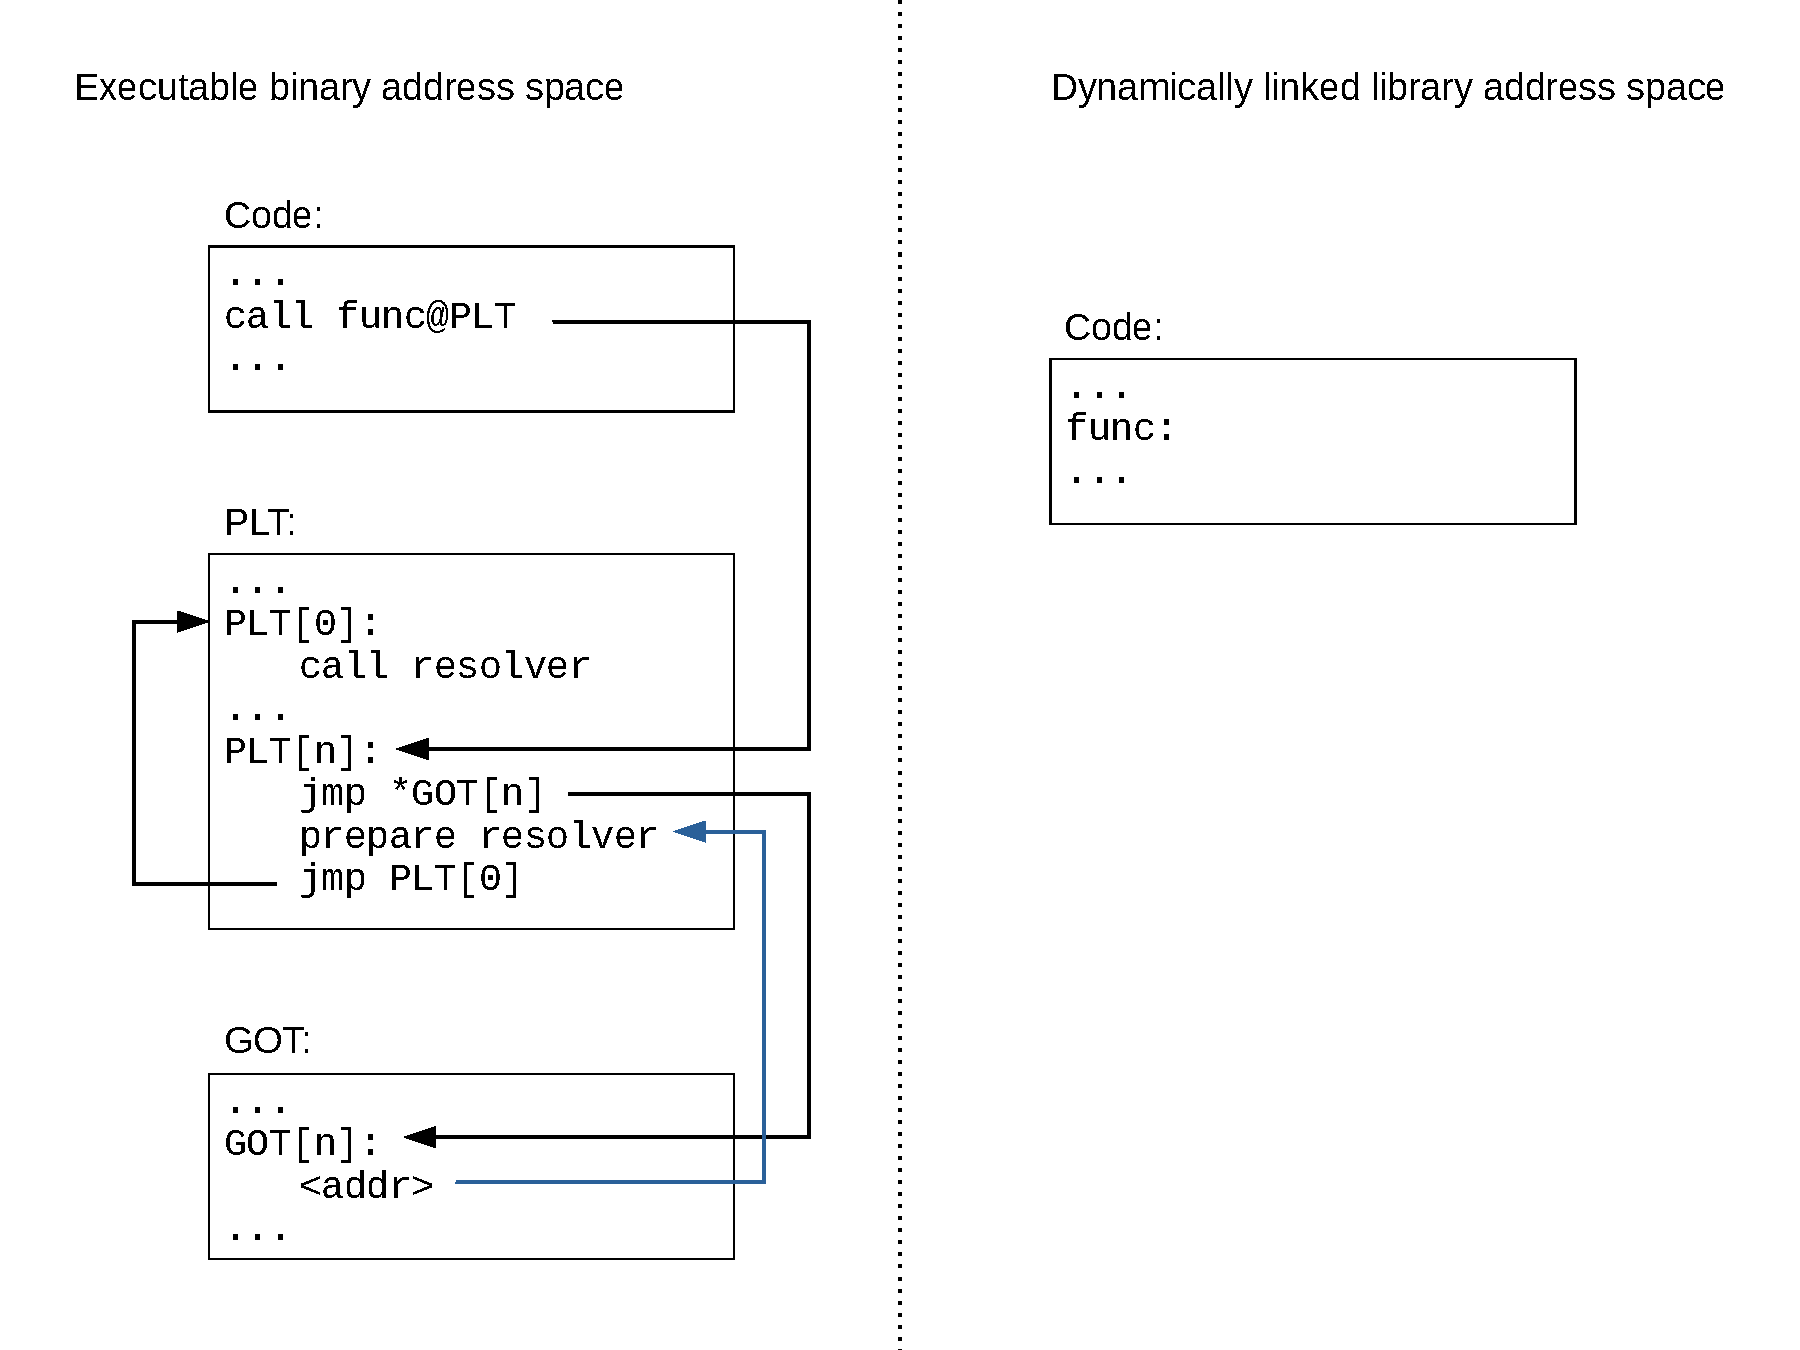
\includegraphics[width=\textwidth]{figures/lazy-binding-1}
		\caption{Function call on first call (own representation based on \cite{Bendersky2011})}
		\label{fig:lazy-binding-1}
	\end{subfigure}
	\hfill
	\begin{subfigure}[t]{0.49\textwidth}
		\centering
		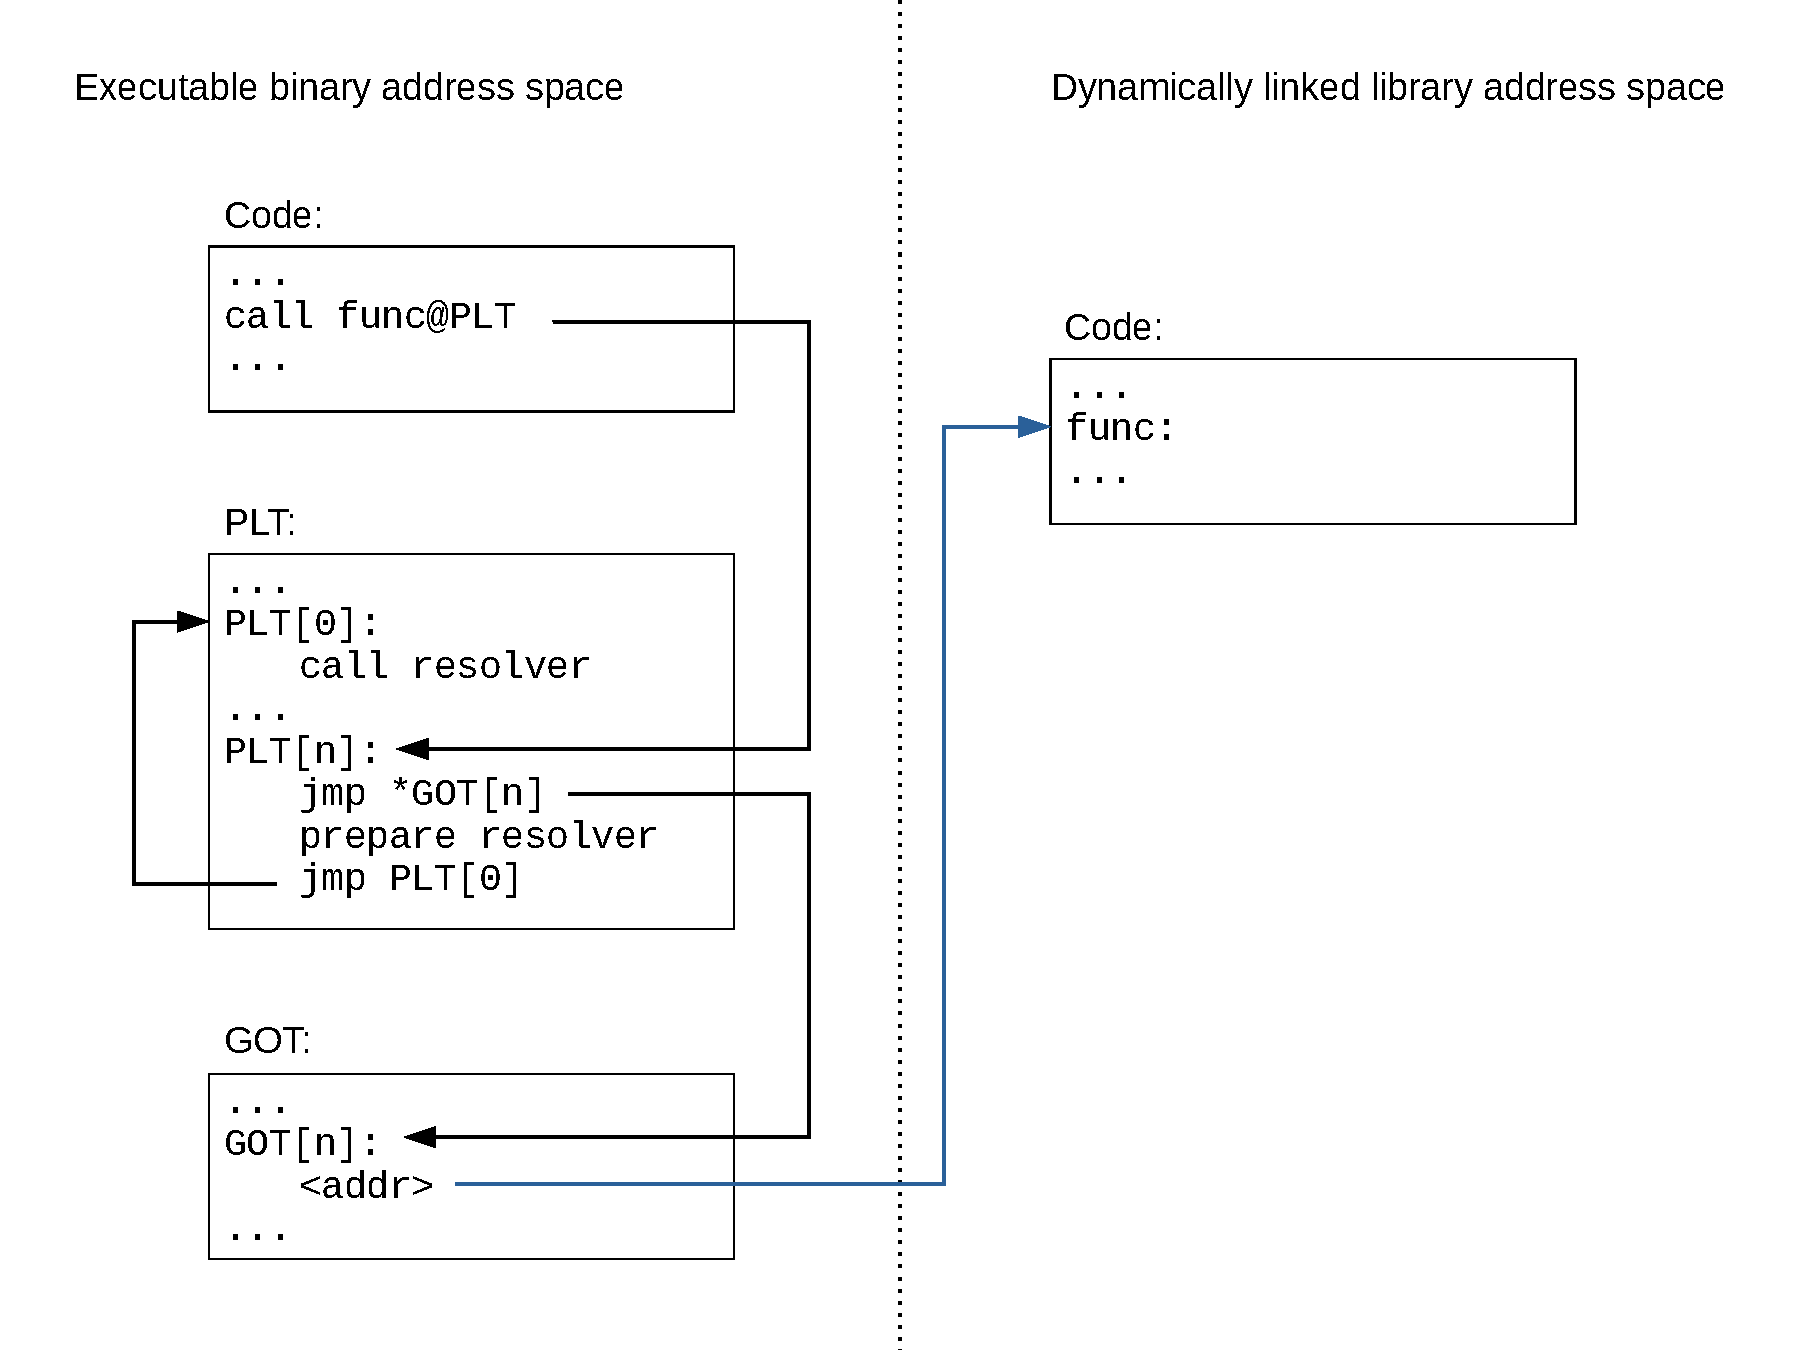
\includegraphics[width=\textwidth]{figures/lazy-binding-2}
		\caption{Function call on subsequent calls (own representation based on \cite{Bendersky2011})}
		\label{fig:lazy-binding-2}
	\end{subfigure}
	\caption{Function call procedure with \acs{plt} and \acs{got} (pseudo-code based on \texttt{x86(\_64)} assembly)}
	\label{fig:lazy-binding}
\end{figure}
